% Options for packages loaded elsewhere
\PassOptionsToPackage{unicode}{hyperref}
\PassOptionsToPackage{hyphens}{url}
%
\documentclass[
  10pt,
]{article}
\usepackage{amsmath,amssymb}
\usepackage{iftex}
\ifPDFTeX
  \usepackage[T1]{fontenc}
  \usepackage[utf8]{inputenc}
  \usepackage{textcomp} % provide euro and other symbols
\else % if luatex or xetex
  \usepackage{unicode-math} % this also loads fontspec
  \defaultfontfeatures{Scale=MatchLowercase}
  \defaultfontfeatures[\rmfamily]{Ligatures=TeX,Scale=1}
\fi
\usepackage{lmodern}
\ifPDFTeX\else
  % xetex/luatex font selection
  \setmainfont[]{DejaVu Serif}
  \setmonofont[]{DejaVu Sans Mono}
\fi
% Use upquote if available, for straight quotes in verbatim environments
\IfFileExists{upquote.sty}{\usepackage{upquote}}{}
\IfFileExists{microtype.sty}{% use microtype if available
  \usepackage[]{microtype}
  \UseMicrotypeSet[protrusion]{basicmath} % disable protrusion for tt fonts
}{}
\makeatletter
\@ifundefined{KOMAClassName}{% if non-KOMA class
  \IfFileExists{parskip.sty}{%
    \usepackage{parskip}
  }{% else
    \setlength{\parindent}{0pt}
    \setlength{\parskip}{6pt plus 2pt minus 1pt}}
}{% if KOMA class
  \KOMAoptions{parskip=half}}
\makeatother
\usepackage{xcolor}
\usepackage[margin=0.65in]{geometry}
\usepackage{longtable,booktabs,array}
\usepackage{calc} % for calculating minipage widths
% Correct order of tables after \paragraph or \subparagraph
\usepackage{etoolbox}
\makeatletter
\patchcmd\longtable{\par}{\if@noskipsec\mbox{}\fi\par}{}{}
\makeatother
% Allow footnotes in longtable head/foot
\IfFileExists{footnotehyper.sty}{\usepackage{footnotehyper}}{\usepackage{footnote}}
\makesavenoteenv{longtable}
\usepackage{graphicx}
\makeatletter
\def\maxwidth{\ifdim\Gin@nat@width>\linewidth\linewidth\else\Gin@nat@width\fi}
\def\maxheight{\ifdim\Gin@nat@height>\textheight\textheight\else\Gin@nat@height\fi}
\makeatother
% Scale images if necessary, so that they will not overflow the page
% margins by default, and it is still possible to overwrite the defaults
% using explicit options in \includegraphics[width, height, ...]{}
\setkeys{Gin}{width=\maxwidth,height=\maxheight,keepaspectratio}
% Set default figure placement to htbp
\makeatletter
\def\fps@figure{htbp}
\makeatother
\setlength{\emergencystretch}{3em} % prevent overfull lines
\providecommand{\tightlist}{%
  \setlength{\itemsep}{0pt}\setlength{\parskip}{0pt}}
\setcounter{secnumdepth}{-\maxdimen} % remove section numbering
\emergencystretch=3em
\sloppy
\ifLuaTeX
  \usepackage{selnolig}  % disable illegal ligatures
\fi
\usepackage{bookmark}
\IfFileExists{xurl.sty}{\usepackage{xurl}}{} % add URL line breaks if available
\urlstyle{same}
\hypersetup{
  hidelinks,
  pdfcreator={LaTeX via pandoc}}

\author{}
\date{}

\begin{document}

\section{Twist-assisted IC: experiment
program}\label{twist-assisted-ic-experiment-program}

Date: 2026-10-21. Scope: pursue routes 1--3 and their combinations,
devise discriminating experiments, and preserve adjacent conditional
routes without claiming an algorithm or novelty.

This program extends
\href{https://github.com/aburan28/crypto/pull/2380}{PR \#2380} and the
\href{../notes/index-calculus/RESEARCH_TWIST_IC_ROUTES_1_3.md}{central
tracker}. It does not substitute an unexecuted plan for measured
results. Bounded native panels have now run; the
\href{reports/EXECUTION_RESULTS.md}{execution results} separate verified
finite checks, partial measurements and remaining
construction/validation gaps. The original acceptance criteria below are
retained.

\subsection{Questions and
deliverables}\label{questions-and-deliverables}

\begin{longtable}[]{@{}
  >{\raggedright\arraybackslash}p{(\columnwidth - 4\tabcolsep) * \real{0.3333}}
  >{\raggedright\arraybackslash}p{(\columnwidth - 4\tabcolsep) * \real{0.3333}}
  >{\raggedright\arraybackslash}p{(\columnwidth - 4\tabcolsep) * \real{0.3333}}@{}}
\toprule\noalign{}
\begin{minipage}[b]{\linewidth}\raggedright
Requested item
\end{minipage} & \begin{minipage}[b]{\linewidth}\raggedright
Deliverable
\end{minipage} & \begin{minipage}[b]{\linewidth}\raggedright
Status
\end{minipage} \\
\midrule\noalign{}
\endhead
\bottomrule\noalign{}
\endlastfoot
Pursue trace restrictions & Explicit coordinate, slope, norm,
multiplicative and divisor families; E01--E06 & Bounded native
restrictions/censuses executed; broader full-cost criteria open \\
Pursue covers & Explicit C\_c family and complement equations, gluing
alternatives, subgroup/class-map gates; E10--E13 & Ten executable class
transfers checked; destination solver/full cost open \\
Pursue solver symmetry & Four membership encodings, equivalent rational
witnesses, torsion descent and solver panel; E07--E09 & Equivalent
systems and three bounded solver attempts executed; broader grid/full
cost open \\
Pursue combinations & Representation/isogeny ablations and full
factorial pipeline panel; E14--E15 & 1,920 native factorial records;
1,704 exact verified replays; cost calibration open \\
Preserve other angles & Exact pairing applicability and bounded
characteristic-zero lifting ingress; E16--E17 & Public applicability and
bounded lift/pairing controls executed; no NIST transfer supplied \\
Make formula checks reproducible & Independent small Rust crate reusing
the repository identity checker & E00 and nine explicit Lean lemmas
checked; concrete field/group/map bridges remain open \\
Preserve follow-up execution & Three versioned backlog protocols,
machine-readable experiment matrix, graph and report PDF & Results and
receipts recorded; cards remain blocked for unmet full-campaign
criteria \\
\end{longtable}

\subsection{Common mathematical
contract}\label{common-mathematical-contract}

The source remains a declared E/F\_p, characteristic p \textgreater{} 3.
The actual DLP target is the original rational order-r subgroup, not the
larger ambient E(F\_(p²)) group. An x-preserving twist uses d*y²=f(x),
omega²=d a nonsquare. Alternative models carry their explicit
conversion.

The trace is tau=1+pi. Anti-invariant points lie in its kernel. Over an
odd-order rational group, a trace fiber is {[}2\^{}-1{]}T+E\^{}-;
counting all lifts can inflate witness counts while leaving projected
rows unchanged. This is the reason for the exact-F and rational-witness
controls, not a complexity lower bound against all coordinate
algorithms.

\subsubsection{Concrete trace families}\label{concrete-trace-families}

Write S=(u+v\emph{omega,w+z}omega).

\begin{itemize}
\tightlist
\item
  \textbf{Coordinate boxes:} u in U\_H and v in V\_H, with
  U\_H=V\_H=\{0,\ldots,H-1\} and H in \{2,4,8\}; both signs of y and all
  exceptional branches retained.
\item
  \textbf{Slope boxes:} u in U\_H and m=z/v in M\_H, with the v!=0
  branch certified separately. The trace has X=m²-2u. A pure-F\_p
  witness formulation uses the same quartic below, without representing
  an extension point.
\item
  \textbf{Norm families:} u²-dv² in W\_H, optionally intersected with a
  coordinate box; analogous y-norm restrictions are separate arms.
\item
  \textbf{Multiplicative families:} subgroups/power images only at H
  dividing p-1, with the exact image size checked. A parameterization
  with costly membership is not a free small base.
\item
  \textbf{Divisor families:} generic degree-two places versus pure twist
  pairs. Principal divisors of x-x0 are removed before row formation;
  they carry no new class relation.
\end{itemize}

The quartic used in the slope arm is

\[
\Delta_T(m)=m^4-6Xm^2-8Ym-3X^2-4A,\qquad 4dv^2=\Delta_T(m).
\]

The line-intersection identity gives a rational-only formulation with
exactly the same witnesses. E00 checks the polynomial arithmetic; the
group interpretation and exceptional cases remain separate obligations.

\subsubsection{A concrete cover family and its
complement}\label{a-concrete-cover-family-and-its-complement}

Let f(x)=x³+Ax+B and choose c with f(c)!=0. Consider

\[
C_c:\;v^2=f(u^2+c).
\]

The two quotient maps on their affine domains are

\[
(u,v)\longmapsto(u^2+c,v)\in E,\qquad
(u,v)\longmapsto(t,z)=(u^2,uv)\in D_c,
\]

where

\[
D_c:\;z^2=t f(t+c).
\]

For t!=0, put F=f(c), a\_2=3c²+A and

\[
X=F/t+a_2/3,\qquad Y=Fz/t^2.
\]

The short complement coefficients are represented without denominators
by

\[
3A_D=3Ac^2+9Bc-A^2,
\]

\[
27B_D=-27Bc^3+18A^2c^2+27ABc+27B^2+2A^3.
\]

These are candidate explicit model-conversion formulas with a polynomial
preflight, not a certified Jacobian subgroup transfer. Require
nonsingularity, f(c)!=0, characteristic \textgreater3, t!=0 on this
affine chart, separate infinity/ramification charts, and actual
divisor-class maps.

The complement must be checked: compare its trace and j, then construct
an F\_p-isomorphism to the requested twist when claimed. Same j alone
confuses twists; opposite trace alone supplies no explicit map. Preserve
complements that fail the twist test as controls.

For a smooth projective geometrically irreducible C/F\_p, genus g, with
a nonconstant degree-delta map to E, the standard point/fiber bound
gives an order-p image when g and delta are fixed. E13 therefore tests
restrictions and pays for them; embedding the original subgroup in a
larger Jacobian is not itself an advantage.

\subsection{Inputs and selection
rules}\label{inputs-and-selection-rules}

The already registered ordinary prime-order structural fixtures are:

\begin{longtable}[]{@{}lrrrr@{}}
\toprule\noalign{}
Source curve & p & A & B & \#E(F\_p) \\
\midrule\noalign{}
\endhead
\bottomrule\noalign{}
\endlastfoot
icv1-fp6-tm7-fc20da94 & 59 & 1 & 13 & 67 \\
icv1-fp10-t5-192cb216 & 827 & 1 & 15 & 823 \\
\end{longtable}

They test group shape and implementation mechanics, not NIST coefficient
fidelity or scaling. The registered even-order controls
icv1-fp7-t4-0c09e92f and icv1-fp7-t2-4910f2d0 expose 2-primary
assumptions; the odd-composite control icv1-fp8-tm1-1ed3feb7 separates
oddness from primality. Verify all parameters and subgroup choices
rather than importing a generator by bit count.

For later scaling, the proposed train/holdout ladder has prime-field bit
lengths \{8,10,12,14\}, A=-3, ordinary odd prime-order curves, and two
independently generated instances per rung. Freeze the generator, all
rejected candidates, registered ICV1/EC1 representations, extension
moduli, generators, exact fixture files and SHA-256 hashes in an
amendment before timing. No such larger fixtures have been generated or
admitted by this plan.

Stage panels use H in \{2,4,8\}, arity m in \{2,3,4\}, projected base
budgets B in \{8,12,16\}, and declared seeds 0--3 for design and 4--7
for holdout. Unsupported and empty cells stay explicit. The resource
envelope and expected cost need calibration before readiness; these
grids are design inputs, not an authorization to launch a paid campaign.

Tiny exact-census cells enumerate every nonidentity rational target plus
a separate identity branch. A performance cell is one previously unseen
public target, with target generation excluded symmetrically from the
online intervals. Planted decompositions are correctness controls only.
Do not use their yield as a uniform-target estimate.

\subsection{Experiment matrix}\label{experiment-matrix}

The canonical machine-readable version is \url{experiments.json}. Every
row below names a falsifier and what its outcome would change.

\subsubsection{E00 --- Polynomial
preflight}\label{e00-polynomial-preflight}

\begin{itemize}
\tightlist
\item
  \textbf{Route / status:} common / verified polynomial preflight and
  five Lean polynomial lemmas; concrete group/map bridges remain open.
\item
  \textbf{Question:} Do the proposed trace and complement coordinate
  formulas satisfy their exact cleared-denominator polynomial
  identities?
\item
  \textbf{Arms and inputs:} Five compiled statement ASTs; exact integer
  coefficient expansion and repository identity certificates;
  deliberately false +1 variants.
\item
  \textbf{Controls:} Exact expansion and modular evaluation are
  different arithmetic checks; all negative variants must reject.
\item
  \textbf{Measurements / acceptance:} All five exact coefficient
  differences zero; 32 issuer and 32 domain-separated checker points
  pass; five false variants reject.
\item
  \textbf{Stop, null outcome and next decision:} Any mismatch stops use
  of the affected formula; no transfer or performance claim follows from
  passing.
\item
  \textbf{Prerequisites:} source and E00 protocol frozen before
  execution.
\end{itemize}

\subsubsection{E01 --- Trace fibers and
separation}\label{e01-trace-fibers-and-separation}

\begin{itemize}
\tightlist
\item
  \textbf{Route / status:} 1 / verified exhaustive bounded fixture
  census; general formal bridge open.
\item
  \textbf{Question:} Which apparent relation gains are just multiple
  lifts of the same trace?
\item
  \textbf{Arms and inputs:} All points on the two registered
  odd-prime-order toy curves over the declared quadratic extension; add
  separate registered even-order and odd-composite controls.
\item
  \textbf{Controls:} Rational-only traces; pure twist trace zero; S+U
  with U in ker(tau); identity; rational 2-primary cases.
\item
  \textbf{Measurements / acceptance:} Exact trace image/fiber counts,
  distinct projected rows, row ranks and target-row span.
\item
  \textbf{Stop, null outcome and next decision:} Do not count repeated
  fibers as new information; a failed asserted identity is a correctness
  failure, not a performance loss.
\item
  \textbf{Prerequisites:} registered exact extension models and native
  point verifier.
\end{itemize}

\subsubsection{E02 --- Coordinate boxes}\label{e02-coordinate-boxes}

\begin{itemize}
\tightlist
\item
  \textbf{Route / status:} 1 / partial: declared restrictions executed;
  full larger-field norm-y/power families open.
\item
  \textbf{Question:} Do small coordinate boxes create a useful small
  trace base with cheaper membership or decomposition?
\item
  \textbf{Arms and inputs:} S=(u+v omega,w+z omega) with u in U and v in
  V; H in \{2,4,8\}; enumerate both y signs and branches.
\item
  \textbf{Controls:} Exact-image rational base; same-size hash-selected
  rational base; unrestricted lift control.
\item
  \textbf{Measurements / acceptance:} Distinct traces, nonzero coverage,
  fiber multiplicities, construction/encoding cost and verified
  independent rows.
\item
  \textbf{Stop, null outcome and next decision:} Record empty bases and
  size collisions; never normalize away construction or
  duplicate-removal work.
\item
  \textbf{Prerequisites:} E01.
\end{itemize}

\subsubsection{E03 --- Slope and real-part
restrictions}\label{e03-slope-and-real-part-restrictions}

\begin{itemize}
\tightlist
\item
  \textbf{Route / status:} 1+3 / verified 30 finite witness-set
  comparisons; cost comparison open.
\item
  \textbf{Question:} Does restricting u and m=z/v help beyond a rational
  parametrization of X=m\^{}2-2u?
\item
  \textbf{Arms and inputs:} u in U and m in M, H in \{2,4,8\}; enforce
  4dv\^{}2=Delta\_T(m); add independent v restriction as an ablation.
\item
  \textbf{Controls:} Same quartic witness written entirely over Fp;
  exact-F table; ordinary low-degree addition witnesses.
\item
  \textbf{Measurements / acceptance:} Projected solution-set equality
  first; then encoding size and counted work per independent row.
\item
  \textbf{Stop, null outcome and next decision:} If the candidate and
  rational witness systems are identical after renaming, classify the
  result as encoding reuse rather than new twist geometry.
\item
  \textbf{Prerequisites:} E01.
\end{itemize}

\subsubsection{E04 --- Norm and multiplicative
restrictions}\label{e04-norm-and-multiplicative-restrictions}

\begin{itemize}
\tightlist
\item
  \textbf{Route / status:} 1 / partial: norm/image controls executed;
  larger-field fibers and costing open.
\item
  \textbf{Question:} Can norm constraints or multiplicative structure
  reduce solve cost after parameterization and membership are charged?
\item
  \textbf{Arms and inputs:} Norm(x)=u\textsuperscript{2-dv}2 in W;
  norm(y) restrictions; H-th-power or subgroup conditions only when H
  divides p-1; intersect with a trace-box family.
\item
  \textbf{Controls:} Same F without norm witnesses; same-size rational
  base; matched subgroup-size control; nonsquare d rescaling.
\item
  \textbf{Measurements / acceptance:} Image size, membership
  degree/selector size, projection collisions and complete stage work.
\item
  \textbf{Stop, null outcome and next decision:} Unchanged projected
  sets at unchanged or higher cost close only that restriction; missing
  roots do not count as a win.
\item
  \textbf{Prerequisites:} E01.
\end{itemize}

\subsubsection{E05 --- Divisors and degree-two
places}\label{e05-divisors-and-degree-two-places}

\begin{itemize}
\tightlist
\item
  \textbf{Route / status:} 1+2 / partial: two sparse-function/divisor
  controls; unsplit degree 3/4 factors open.
\item
  \textbf{Question:} Can generic conjugate pairs help smooth-divisor
  relations when the principal pure-twist pairs are removed?
\item
  \textbf{Arms and inputs:} Sparse rational functions a(x)+y b(x),
  coefficient support frozen; distinguish x in Fp from genuinely
  nonrational degree-two places.
\item
  \textbf{Controls:} Remove divisors of x-x0 before forming rows;
  rational-only function family; generic degree-two-place control.
\item
  \textbf{Measurements / acceptance:} Factoring and lifting work,
  nontrivial projected divisor rows, row span and failed factorizations.
\item
  \textbf{Stop, null outcome and next decision:} Principal pairs and
  empty projected rows are not relations; retain the full degree and
  coefficient-height budgets.
\item
  \textbf{Prerequisites:} E01; native divisor and factorization
  verifier.
\end{itemize}

\subsubsection{E06 --- Exact relation
census}\label{e06-exact-relation-census}

\begin{itemize}
\tightlist
\item
  \textbf{Route / status:} 1+3 / partial: 1179 configured census rows,
  678 verified and 501 unsupported; decomposition cost open.
\item
  \textbf{Question:} Which restricted bases actually span the needed
  target rows?
\item
  \textbf{Arms and inputs:} m in \{2,3,4\}, B in \{8,12,16\}; all
  nonidentity targets for tiny fixtures; freeze sign/orbit conventions.
\item
  \textbf{Controls:} Complete enumeration or MITM oracle; identical
  projected base and target; raw versus canonicalized rows.
\item
  \textbf{Measurements / acceptance:} Exact relation set, target
  coverage, rank over r, target-row span and verified known-answer
  recovery.
\item
  \textbf{Stop, null outcome and next decision:} Do not silently replace
  unattainable full-column rank with a new stopping rule; freeze
  target-span stopping in advance.
\item
  \textbf{Prerequisites:} E02 or E03 or E04.
\end{itemize}

\subsubsection{E07 --- Equivalent system
builders}\label{e07-equivalent-system-builders}

\begin{itemize}
\tightlist
\item
  \textbf{Route / status:} 3 / partial: 240 distinct B8/H8 projection
  cells verified; B12/16 and other bases open.
\item
  \textbf{Question:} Which membership representation avoids merely
  moving cost into a higher-degree constraint?
\item
  \textbf{Arms and inputs:} Univariate product membership, bit
  decomposition with proven range, selector/product chains and explicit
  branching.
\item
  \textbf{Controls:} Untwisted addition chain; exact same projected F;
  independently enumerated projected solutions.
\item
  \textbf{Measurements / acceptance:} Equality of full projected sets
  including multiplicity/sign policy and exceptional branches;
  equations/variables/degrees.
\item
  \textbf{Stop, null outcome and next decision:} A mismatch blocks all
  solver comparisons until repaired; coefficient fields and modular-wrap
  conditions are part of the input.
\item
  \textbf{Prerequisites:} E06.
\end{itemize}

\subsubsection{E08 --- Solver and ordering
panel}\label{e08-solver-and-ordering-panel}

\begin{itemize}
\tightlist
\item
  \textbf{Route / status:} 3 / partial: three 1930-cell bounded solver
  attempts retained; applicable signature reference, broader grid and
  full costs open.
\item
  \textbf{Question:} Does symmetry reduce actual solving cost against
  the strongest equivalent encoding?
\item
  \textbf{Arms and inputs:} Frozen variable orders,
  chain/quadratized/symmetric encodings; msolve/open reference plus
  available applicable F4/F5 engines.
\item
  \textbf{Controls:} A/A runs; untwisted witness system;
  redundant-variable positive/negative controls; same output verifier.
\item
  \textbf{Measurements / acceptance:} Counted native operations,
  Macaulay dimensions/nnz, reductions, solving degree, memory, failures
  and cost per useful row.
\item
  \textbf{Stop, null outcome and next decision:} Lower displayed degree
  alone is not a win; timeouts and OOMs remain incomplete outcomes under
  the same envelope.
\item
  \textbf{Prerequisites:} E07; calibrated external-solver adapters.
\end{itemize}

\subsubsection{E09 --- Torsion over
extensions}\label{e09-torsion-over-extensions}

\begin{itemize}
\tightlist
\item
  \textbf{Route / status:} 1+3 / verified bounded translated-torsion
  controls; general proof bridge open.
\item
  \textbf{Question:} Can torsion symmetry survive Galois descent without
  false factor-base compression?
\item
  \textbf{Arms and inputs:} 2-torsion over Fp\^{}3 and combined Fp\^{}6
  where applicable; Galois-invariant coordinates and descent
  constraints.
\item
  \textbf{Controls:} No-torsion encoding; {[}2{]} map on the odd
  subgroup; retained extension-field cost; rational torsion
  special-family control.
\item
  \textbf{Measurements / acceptance:} Equivalence, actual orbit/image
  size, descended system degree and complete representation cost.
\item
  \textbf{Stop, null outcome and next decision:} A geometric torsion
  orbit that leaves the rational base is not a rational factor-base
  quotient.
\item
  \textbf{Prerequisites:} E07; registered extension models and torsion
  verification.
\end{itemize}

\subsubsection{E10 --- Explicit degree-two
covers}\label{e10-explicit-degree-two-covers}

\begin{itemize}
\tightlist
\item
  \textbf{Route / status:} 2 / verified exhaustive declared-family
  search over 27140 parameters on ten fixtures.
\item
  \textbf{Question:} When is the complementary elliptic quotient
  actually the required twist?
\item
  \textbf{Arms and inputs:} C\_c: v\textsuperscript{2=f(u}2+c), f(c)!=0;
  quotient E and D\_c: z\^{}2=t f(t+c); use the explicit short
  complement coefficients.
\item
  \textbf{Controls:} Reject f(c)=0; same-j only control; trace-opposite
  only control; explicit Fp isomorphism check.
\item
  \textbf{Measurements / acceptance:} Smoothness/genus, complete
  quotient maps including infinity, complement trace/j, isomorphism and
  image size.
\item
  \textbf{Stop, null outcome and next decision:} Neither matching j nor
  opposite trace alone certifies the requested isomorphism or subgroup
  transfer.
\item
  \textbf{Prerequisites:} E00; native smoothness and map checker.
\end{itemize}

\subsubsection{E11 --- Gluing and alternative
complements}\label{e11-gluing-and-alternative-complements}

\begin{itemize}
\tightlist
\item
  \textbf{Route / status:} 2 / partial: module filters and two-cover
  search; three positive toy module cases and the public P-521 module
  filter need actual torsion/polarization/quotient/map constructions.
\item
  \textbf{Question:} Do other gluing orders or complementary-factor
  constructions provide a better executable route?
\item
  \textbf{Arms and inputs:} Galois-equivariant 2/3-torsion gluing where
  applicable; recover the complement from a supplied cover; bounded
  typed candidate families.
\item
  \textbf{Controls:} Degenerate/product polarization control;
  incompatible Frobenius control; identical-field checks.
\item
  \textbf{Measurements / acceptance:} Actual curve/map construction,
  indecomposable polarization, subgroup kernel, factored evaluation cost
  and failures.
\item
  \textbf{Stop, null outcome and next decision:} A rejected family or
  failed bounded search does not establish universal nonexistence.
\item
  \textbf{Prerequisites:} E10; gluing/complement implementation.
\end{itemize}

\subsubsection{E12 --- Jacobian arithmetic and
recovery}\label{e12-jacobian-arithmetic-and-recovery}

\begin{itemize}
\tightlist
\item
  \textbf{Route / status:} 2 / partial: ten executable transfers, 5855
  classes, independent PARI orders; formal/independent-host class-map
  bridge open.
\item
  \textbf{Question:} Does the proposed transfer work on the divisor
  classes the collector actually produces?
\item
  \textbf{Arms and inputs:} Pullback/norm on the chosen infinity model;
  arbitrary valid reduced classes; image subgroup order and recovery.
\item
  \textbf{Controls:} phi\_\emph{phi\^{}}={[}degree{]}; origin and
  ramified fibers; independent CAS; direct-E solver.
\item
  \textbf{Measurements / acceptance:} Exact group-law and
  kernel/recovery checks; separate setup, maps, arithmetic and recovery
  costs.
\item
  \textbf{Stop, null outcome and next decision:} Unsupported
  two-infinity or arbitrary-class arithmetic remains unsupported, not
  approximated by rational point-class tests.
\item
  \textbf{Prerequisites:} E10 or E11; native divisor-class arithmetic
  and norm.
\end{itemize}

\subsubsection{E13 --- Restricted cover
images}\label{e13-restricted-cover-images}

\begin{itemize}
\tightlist
\item
  \textbf{Route / status:} 1+2 / partial: low-height image census;
  Jacobian decomposition and useful-row cost open.
\item
  \textbf{Question:} Can restricting cover points give a small base
  without a worse membership or map problem?
\item
  \textbf{Arms and inputs:} All-C(Fp) control; restricted u/trace/norm
  supports; degree/genus ladder only with frozen factored maps.
\item
  \textbf{Controls:} Same projected base on E; fixed-genus image bound;
  independent point counts.
\item
  \textbf{Measurements / acceptance:} Actual image size,
  g/degree/representation size, construction and membership cost,
  projected rows.
\item
  \textbf{Stop, null outcome and next decision:} A fixed bounded-degree
  cover with order-p image does not supply a small base merely by
  changing the ambient variety.
\item
  \textbf{Prerequisites:} E12.
\end{itemize}

\subsubsection{E14 --- Model and isogeny
ablations}\label{e14-model-and-isogeny-ablations}

\begin{itemize}
\tightlist
\item
  \textbf{Route / status:} 1+2+3 / verified bounded map/dual
  construction: three explicit degree-seven maps and all three algebraic
  duals in V2; full IC costs open.
\item
  \textbf{Question:} Are any savings due to cheaper constants or another
  isogenous representative rather than new relations?
\item
  \textbf{Arms and inputs:} Nonsquare d choices, x-preserving/standard
  twist models, fixed small-degree rational isogeny routes and verified
  return maps.
\item
  \textbf{Controls:} Equivalent direct-E representation; same source
  target/subgroup; conversion charged both ways.
\item
  \textbf{Measurements / acceptance:} Identical recovered outputs and
  projected relation policy; map, primitive and solver cost separated.
\item
  \textbf{Stop, null outcome and next decision:} Different j or field
  models require typed identities; do not infer an unknown-scalar
  speedup from faster known-scalar multiplication.
\item
  \textbf{Prerequisites:} E07; verified map adapters.
\end{itemize}

\subsubsection{E15 --- Factorial pipeline
ablation}\label{e15-factorial-pipeline-ablation}

\begin{itemize}
\tightlist
\item
  \textbf{Route / status:} 1+2+3 / partial: 1920 native records, 1704
  verified and identically replayed, 216 empty-base errors; calibrated
  full cost and independent host open.
\item
  \textbf{Question:} Which component or combination improves the actual
  IC baseline?
\item
  \textbf{Arms and inputs:} Trace restriction on/off, cover on/off,
  solver symmetry on/off; pairs use equal target/base or explicitly
  separate changed-base studies.
\item
  \textbf{Controls:} Strongest current IC baseline; strongest
  same-target rho; direct destination generic solver; independent
  holdouts.
\item
  \textbf{Measurements / acceptance:} Cold single-target complete
  counted cost and S; setup/online split; 0/0.1/1 GAE pricing band;
  verification and replay.
\item
  \textbf{Stop, null outcome and next decision:} Every claimed IC
  improvement needs baseline/candidate \textgreater1 with all phases;
  rho is a reported gap, not the IC improvement pass gate.
\item
  \textbf{Prerequisites:} E06; E08; E12 for cover cells.
\end{itemize}

\subsubsection{E16 --- Homomorphism and pairing
applicability}\label{e16-homomorphism-and-pairing-applicability}

\begin{itemize}
\tightlist
\item
  \textbf{Route / status:} conditional / verified fifteen
  public-parameter checks and known degree-two pairing positive control;
  no NIST transfer supplied.
\item
  \textbf{Question:} Do small twist factors or a pairing actually supply
  an admissible transfer on the original subgroup?
\item
  \textbf{Arms and inputs:} Exact gcd(r,\#E\_tw), embedding-degree and
  torsion/Frobenius tests on the declared public parameters.
\item
  \textbf{Controls:} Trace/norm killing pure anti-invariants;
  translated-coset control; known small-embedding-degree positive family
  kept separate.
\item
  \textbf{Measurements / acceptance:} Exact applicability certificates
  and a named nondegenerate transfer if one exists.
\item
  \textbf{Stop, null outcome and next decision:} A smooth twist order or
  shared x-coordinate relation does not supply a subgroup-preserving
  transfer; do not run a nonexistent destination attack.
\item
  \textbf{Prerequisites:} exact public-parameter and transfer checker.
\end{itemize}

\subsubsection{E17 --- Arithmetic lift and twist
ingress}\label{e17-arithmetic-lift-and-twist-ingress}

\begin{itemize}
\tightlist
\item
  \textbf{Route / status:} conditional / partial: integral and two
  254-case rational-height panels; one rank interval, target lifting and
  discovery cost open.
\item
  \textbf{Question:} Could a characteristic-zero twist reduce to E while
  providing a usable small-height relation source?
\item
  \textbf{Arms and inputs:} Only twists whose parameter is square mod p
  for a same-E reduction; bounded height/rank/search families stated
  before a pilot.
\item
  \textbf{Controls:} Nonsquare reduction goes to the other finite-field
  component; fixed-lift and equal-height controls; charge discovery and
  target lifting.
\item
  \textbf{Measurements / acceptance:} Explicit reduction map, target
  lift, relation independence, heights and construction/search costs
  before any solver comparison.
\item
  \textbf{Stop, null outcome and next decision:} High rank alone is not
  a cheap target lift or a speedup; no unbounded rank or designer-secret
  assumption is treated as evidence.
\item
  \textbf{Prerequisites:} separate arithmetic-lift construction and
  height protocol.
\end{itemize}

\subsection{Fair comparisons and
attribution}\label{fair-comparisons-and-attribution}

Run three controls when a candidate provides an image F:

\begin{enumerate}
\def\labelenumi{\arabic{enumi}.}
\tightlist
\item
  \textbf{Exact-F table:} materialize the identical projected point set
  and charge construction/storage.
\item
  \textbf{Rational witness:} retain every useful F\_p auxiliary
  parameter and the same quartic/membership constraints; remove only the
  extension-field interpretation.
\item
  \textbf{Strong ordinary IC baseline:} the best applicable verified
  pipeline with its own fair tuning budget, plus a matched strong rho
  reference.
\end{enumerate}

A candidate losing its apparent advantage against control 2 has not
discovered a benefit from twist relations. It may still be a useful
encoding optimization, which is reported against the previous IC
baseline. If a cover changes F, either compare paired arms on the same F
or declare a separate changed-base experiment; an eight-cell factorial
design cannot assume unrelated workloads match.

Membership is part of the problem. Compare product polynomials, bounded
bit decompositions, selector/product chains and explicit branch
enumeration with all selection, range and modular-wrap checks charged. A
high-degree membership constraint cannot be omitted from the solver
input.

Use canonical signed/orbit representatives only under a proved rule.
Count projected nontrivial coefficient rows, their rank and the
target-row span. Duplicate lifts, zero rows and scalar/multiple rows
stay in the raw evidence and are not called independent relations. Full
column rank is not silently assumed; target recoverability and the
stopping rule are frozen before execution.

\subsection{Success, stopping and cost}\label{success-stopping-and-cost}

The immediate success criterion is a verified lower cost against the
best current IC baseline on identical accepted workloads. For a stage,
compare counted cost per independent useful projected row and label it a
stage result. For a full pipeline, report
baseline\_total/candidate\_total \textgreater1 with every phase
included. A rho crossover is a separate claim requiring the same target,
complete intervals and the strongest applicable rho implementation.

Use the repository's single-target ecbench contract for method
comparisons. Report cold cost, setup and online costs separately; retain
attempted and completed counts, verification, failed searches, OOMs and
timeouts. Price uncalibrated work at 0, 0.1 and 1 GAE symmetrically for
all arms. A ranking that changes within this band is unresolved.
Wall-time results additionally require isolation, A/A controls, paired
reruns and admitted uncertainty.

For solver experiments, export exactly the same systems and verify full
projected solution sets before ranking. Compare with the fastest
available applicable external implementation; missing Magma or other
proprietary comparisons are named, not silently replaced by a weaker
reference. Exponents require at least four sizes and full phase costs;
two toy fixtures are not a scaling result.

For an admitted performance comparison, freeze per-cell limits after
cost calibration. The initial L0 diagnostic caps were frozen before
execution, with full calibration still open and no speed claim admitted.
Stop the affected cell on a correctness mismatch. Preserve budget
exhaustion as an incomplete outcome under the original envelope. A null
result closes the tested family only, not every possible twist-related
construction.

\subsection{Dependency and execution
order}\label{dependency-and-execution-order}

\begin{itemize}
\tightlist
\item
  E00 can run after its source and protocol are committed.
\item
  E01 and E10 are independent construction/geometry diagnostics.
\item
  E02--E06 generate and qualify restricted bases; E07 verifies system
  equivalence before E08/E09 timing.
\item
  E11/E12 must establish actual divisor-class maps before E13 or any
  cover-containing E15 cell.
\item
  E14 separates representation costs from relation effects.
\item
  E15 is the final combined pipeline panel; E16/E17 remain conditional
  ingress tests with no assumed transfer.
\item
  Backlog route cards own these phases and remain blocked until their
  actual native drivers/checkers, source pins, resource estimates and
  fixture hashes exist. No unsupported component is marked runnable by
  adding this document.
\end{itemize}

See \url{PROGRAM.svg} for the dependency diagram.

\begin{figure}
\centering
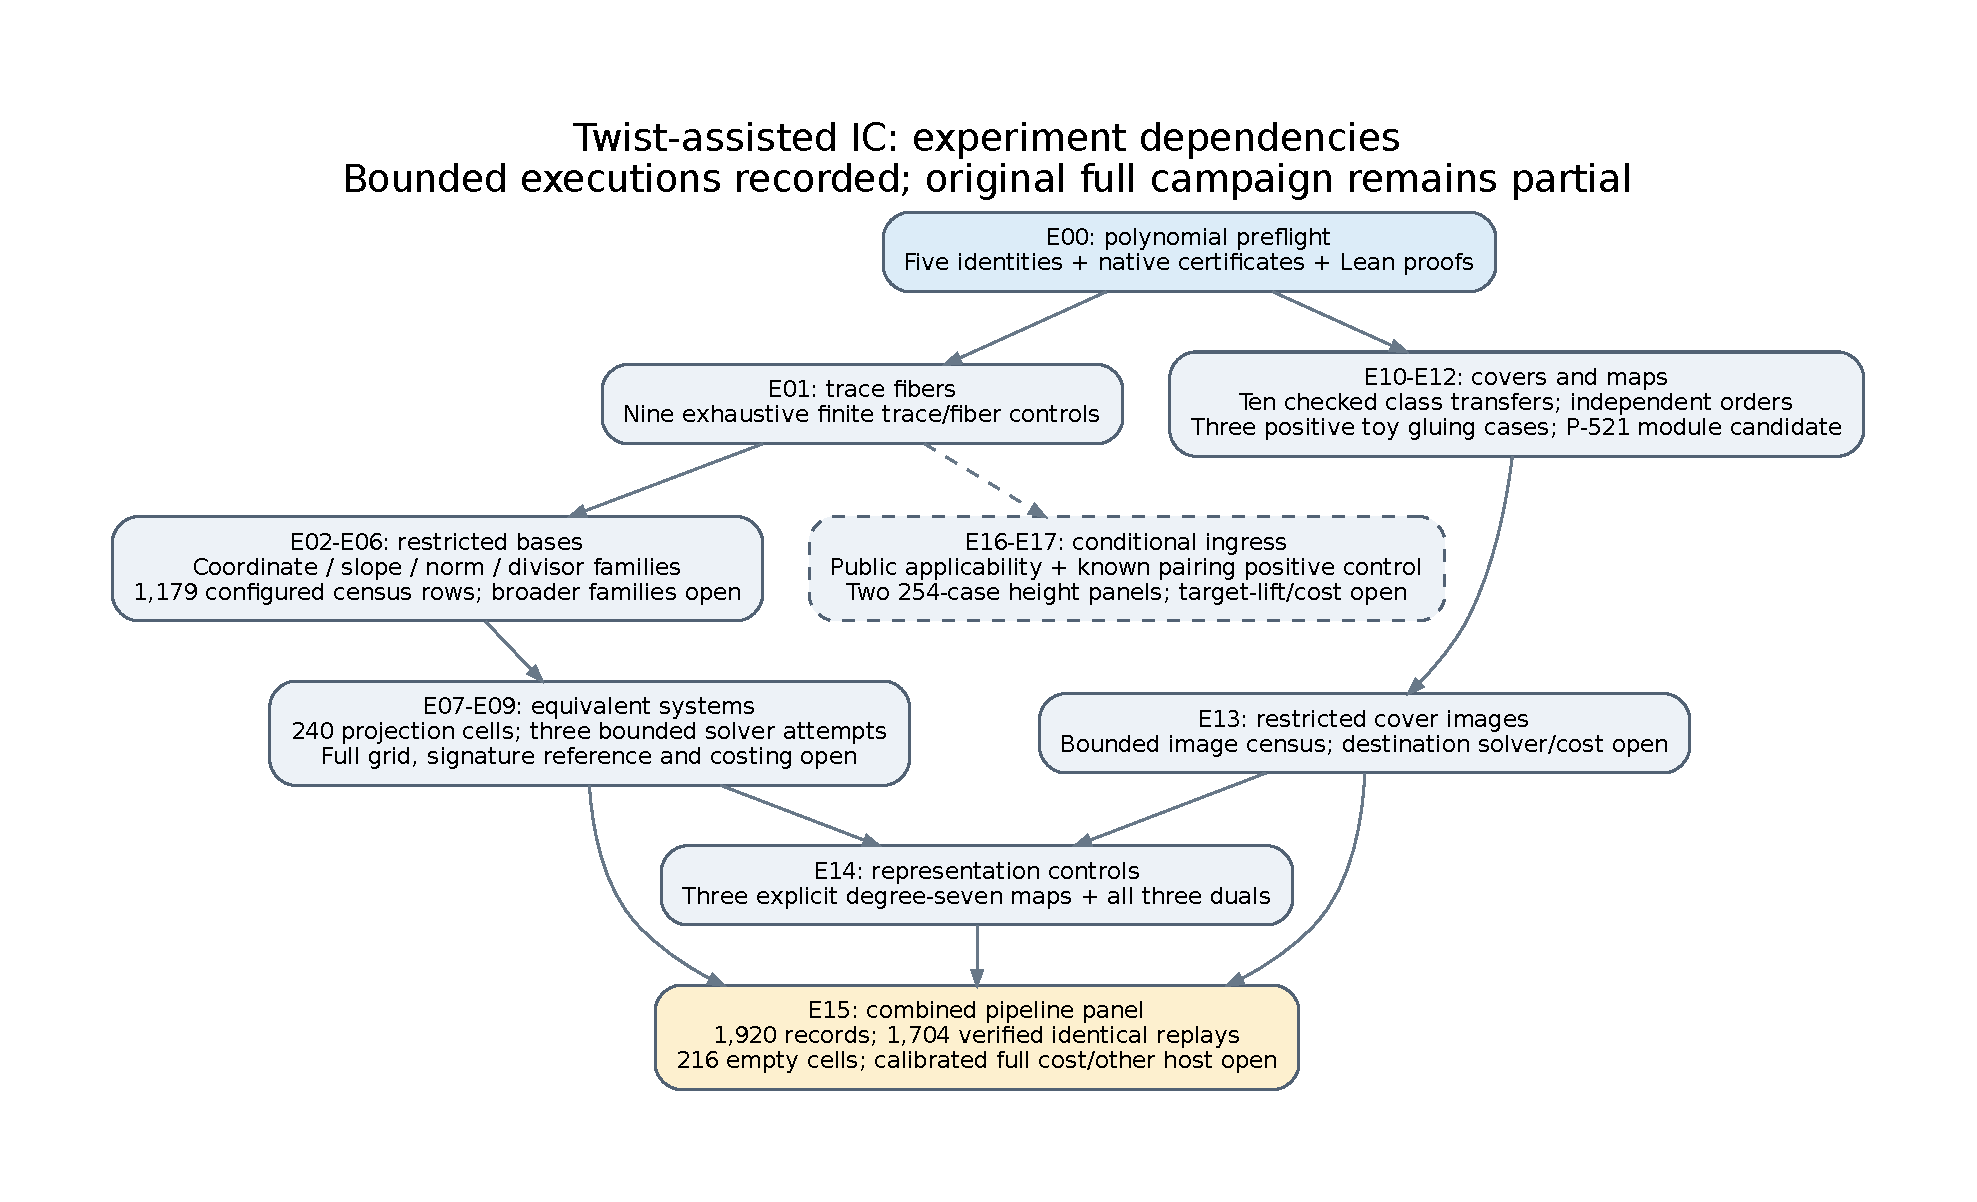
\includegraphics{PROGRAM.pdf}
\caption{Experiment dependencies and bounded execution; the original
full campaign remains partial}
\end{figure}

The PDF includes that same diagram. No performance dashboard value
changes until a result meets the repository validation gate.

\subsection{Proof map and limits}\label{proof-map-and-limits}

\begin{longtable}[]{@{}
  >{\raggedright\arraybackslash}p{(\columnwidth - 4\tabcolsep) * \real{0.3333}}
  >{\raggedright\arraybackslash}p{(\columnwidth - 4\tabcolsep) * \real{0.3333}}
  >{\raggedright\arraybackslash}p{(\columnwidth - 4\tabcolsep) * \real{0.3333}}@{}}
\toprule\noalign{}
\begin{minipage}[b]{\linewidth}\raggedright
Item
\end{minipage} & \begin{minipage}[b]{\linewidth}\raggedright
Check implemented here
\end{minipage} & \begin{minipage}[b]{\linewidth}\raggedright
Remaining proof / execution obligation
\end{minipage} \\
\midrule\noalign{}
\endhead
\bottomrule\noalign{}
\endlastfoot
Chord polynomial division and quartic expansion & E00
coefficient/evaluated certificates and corresponding Lean identities &
Concrete elliptic group and exceptional-chart bridge \\
Complement coefficients and cleared model conversion & E00 arithmetic,
Lean identities and ten executable toy class transfers & Faithful formal
field/chart/Jacobian maps and independent arbitrary-class replay \\
Trace-fiber and separation statements & Nine exhaustive native censuses
and four conditional Weierstrass point-group Lean statements & Concrete
finite-field Frobenius/twist and odd-subgroup bridge \\
Image-size bound & A stated standard bound with explicit hypotheses &
Applicable curve/morphism hypotheses and proof mapping for any selected
candidate \\
Solver equivalence and benefit & 240 distinct projection checks, bounded
solver panels and native IC/replay & Broader grids, complete applicable
external reference and calibrated full costs \\
NIST-size applicability or novelty & Not established & Separate scalable
construction, applicable evidence and a literature novelty audit \\
\end{longtable}

A certificate with proof=null is evaluated-tier, not a Lean proof.
Different checker points in one process do not constitute
independent-host replay. Clearing denominators certifies only a
polynomial identity; it does not prove the original rational map is
defined everywhere.

\subsection{Sources}\label{sources}

\begin{itemize}
\tightlist
\item
  \href{https://eprint.iacr.org/2004/031}{Semaev, summation polynomials,
  ePrint 2004/031}.
\item
  \href{https://www.iacr.org/archive/eurocrypt2014/84410158/84410158.pdf}{Faugere--Huot--Joux--Renault--Vitse,
  torsion symmetries, EUROCRYPT 2014}.
\item
  \href{https://eprint.iacr.org/2011/020}{Joux--Vitse, cover and
  decomposition, ePrint 2011/020}; extension-field results are not a
  NIST prime-field result.
\item
  \href{https://arxiv.org/abs/1403.6911}{Broker--Howe--Lauter--Stevenhagen,
  gluing constructions}.
\item
  \href{https://arxiv.org/abs/2606.02429}{Gallese--Lombardo--Naccarato--Zannier,
  Finding the complement of an elliptic curve inside a Jacobian,
  arXiv:2606.02429v1}. Prior art for computing a complementary factor,
  not an IC speedup.
\item
  \href{../../.agents/skills/ecdlp-surfaces/references/higher-genus.md}{Higher-genus
  implementation contract},
  \href{../../docs/identity-certificates/README.md}{identity certificate
  contract}.
\item
  \href{https://github.com/aburan28/crypto/pull/2368}{PR \#2368},
  unmerged prior mixed-component study at the time this program was
  written; no new replay of its results is claimed here.
\end{itemize}

\subsection{Execution evidence}\label{execution-evidence}

The historical \href{reports/RESULTS.md}{E00 preflight report} checks
five exact polynomial identities and evaluated certificates, rejects
five false variants, and records 22 supporting tests. The subsequent
\href{reports/EXECUTION_RESULTS.md}{bounded execution report} and
per-experiment statuses above record E01--E17 execution/applicability
evidence and every remaining original requirement. No calibrated speedup
or novelty claim follows.

\end{document}
